\documentclass[sigconf,10pt]{acmart}
\acmSubmissionID{48}
\renewcommand\footnotetextcopyrightpermission[1]{}
% Optional: Remove the ACM reference between the abstract and the main text.
\settopmatter{printfolios=true,printacmref=false}
% Optional: Comment out the CCS concepts and keywords.
\usepackage{tikz}
\usepackage{float}
\usepackage{amsmath}
\usepackage{xspace}
\usepackage{cleveref}
\usepackage{balance}
\usepackage{url}
\usepackage{siunitx}
\usepackage{comment}
\usepackage{enumitem}
\usepackage{listings}
\usepackage{minted}
\usepackage{tikz}
\usepackage{subcaption}
\usepackage{lmodern}

\newcommand*\circled[1]{\tikz[baseline=(char.base)]{
            \node[shape=circle,draw=black!80,line width=0.2mm,inner sep=0.1pt] (char) {#1};}}

\newcommand{\sys}{ChainIO\xspace}
\newcommand{\tech}{AdaptiveOffload\xspace}

\newcommand{\eg}{e.g.,\xspace}
\newcommand{\ie}{i.e.,\xspace}
\newcommand{\etc}{etc.\xspace}

% Cleveref formatting
\crefname{algocf}{algorithm}{algorithms}
\Crefname{algocf}{Algorithm}{Algorithms}
\crefformat{section}{\S#2#1#3}
\Crefformat{section}{Section~#2#1#3}
\crefformat{subsection}{\S#2#1#3}
\Crefformat{subsection}{Section~#2#1#3}
\crefformat{subsubsection}{\S#2#1#3}
\Crefformat{subsubsection}{Section~#2#1#3}
\crefformat{figure}{figure~#2#1#3}
\Crefformat{figure}{Figure~#2#1#3}


% Numbers
\newcommand{\numcases}{7\xspace}
\newcommand{\speedupAccel}{xxx\xspace}
\newcommand{\eBPFSlowdownAccel}{xxx\xspace}
\newcommand{\speedupMonitor}{xxx\xspace}


\newlength{\mintednumbersep}
\AtBeginDocument{%
  \sbox0{\tiny00}%
  \setlength\mintednumbersep{\parindent}%
  \addtolength\mintednumbersep{-\wd0}%
}

\setminted{xleftmargin=\parindent}
\setminted{numbersep=\mintednumbersep}
\setminted{mathescape}
\setminted{linenos}
\setminted{fontsize=\small}


%%% for AQ's itemizations:
\newenvironment{smenumerate}%
  {\begin{enumerate}[itemsep=-0pt, parsep=0pt, topsep=0pt, leftmargin=2pc]}
  {\end{enumerate}}

\newenvironment{smitemize}%
  {\begin{list}{$\bullet$}%
    {\setlength{\parsep}{0pt}%
      \setlength{\topsep}{0pt}%
      \setlength{\leftmargin}{2pc}%
      \setlength{\itemsep}{1pt}}}
  {\end{list}}



\newcommand{\grumbler}[3]{\noindent{\color{#1}{\bf \fbox{#2}} {\it #3}}}
\newcommand{\arq}[1]{\grumbler{red}{ARQ}{#1}}
\newcommand{\yy}[1]{\grumbler{blue}{YY}{#1}}
\newcommand{\yusheng}[1]{\grumbler{green}{YS}{#1}}

\newcommand{\todo}[1]{\grumbler{olive}{todo}{#1}}


\title{\sys: Bridging Disk and Network Domains with eBPF}
% anyauthor declaration will be ignored  when using 'pldi' option (for double blind review)
%

% \author{
%     {\rm Yiwei Yang}\\ UC Santa Cruz
% }
\author{
Anonymous Authors
}

\begin{document}

\begin{abstract}
Modern data-driven services like distributed analytical databases incur high tail-latencies because each storage operation (\texttt{read}) and network operation (\texttt{send}/\texttt{recv}) triggers a separate user-kernel crossing. While \texttt{io\_uring} accelerates block I/O and AF\_XDP accelerates packet I/O, no solution chains them end-to-end in a unified framework. We introduce \sys, a hybrid I/O-bypass framework that transparently live-patches POSIX I/O calls into a unified submission queue, and coordinates disk and network operations via shared BPF maps. By chaining these bypass paths with in-kernel eBPF programs, \sys achieves near zero-copy, batched I/O across domains, without modifying application source code. Our preliminary evaluation on ClickHouse TPC-H queries shows up to 4× higher IOPS and 30\% reduction in CPU utilization compared to standalone \texttt{io\_uring} or DPDK-based implementations, all without application changes.
\end{abstract}

\maketitle

\section{Introduction}

Modern data-intensive applications face significant performance bottlenecks due to the cost of repeated user-kernel transitions, exacerbated by Spectre and Meltdown mitigations. Each storage and network operation requires separate syscalls, with aggregate latency reaching hundreds of milliseconds in data-intensive workloads with fan-out patterns. While \texttt{io\_uring} provides asynchronous, batched disk operations, it still requires expensive syscalls for network traffic; conversely, AF\_XDP delivers zero-copy network acceleration but offers nothing for storage access. Previous research has approached this challenge from several angles without fully solving the cross-domain problem: FlexSC~\cite{flexsc} and MegaPipe batch syscalls but focus on single domains, while DPDK/SPDK and Demikernel~\cite{zhang2021demikernel} bypass the kernel entirely but require extensive application modifications. eBPF-based solutions like XRP~\cite{Zhong22} and BPF-oF~\cite{zarkadas2023bpf} accelerate specific I/O paths (NVMe reads, remote storage) without addressing cross-domain dependencies. Even architectural innovations like IX~\cite{ix} that redesign the OS with separate control and data planes remain siloed in network or storage specialization, leaving a critical gap for workloads that chain operations across both domains.

\begin{figure}[h]
\centering
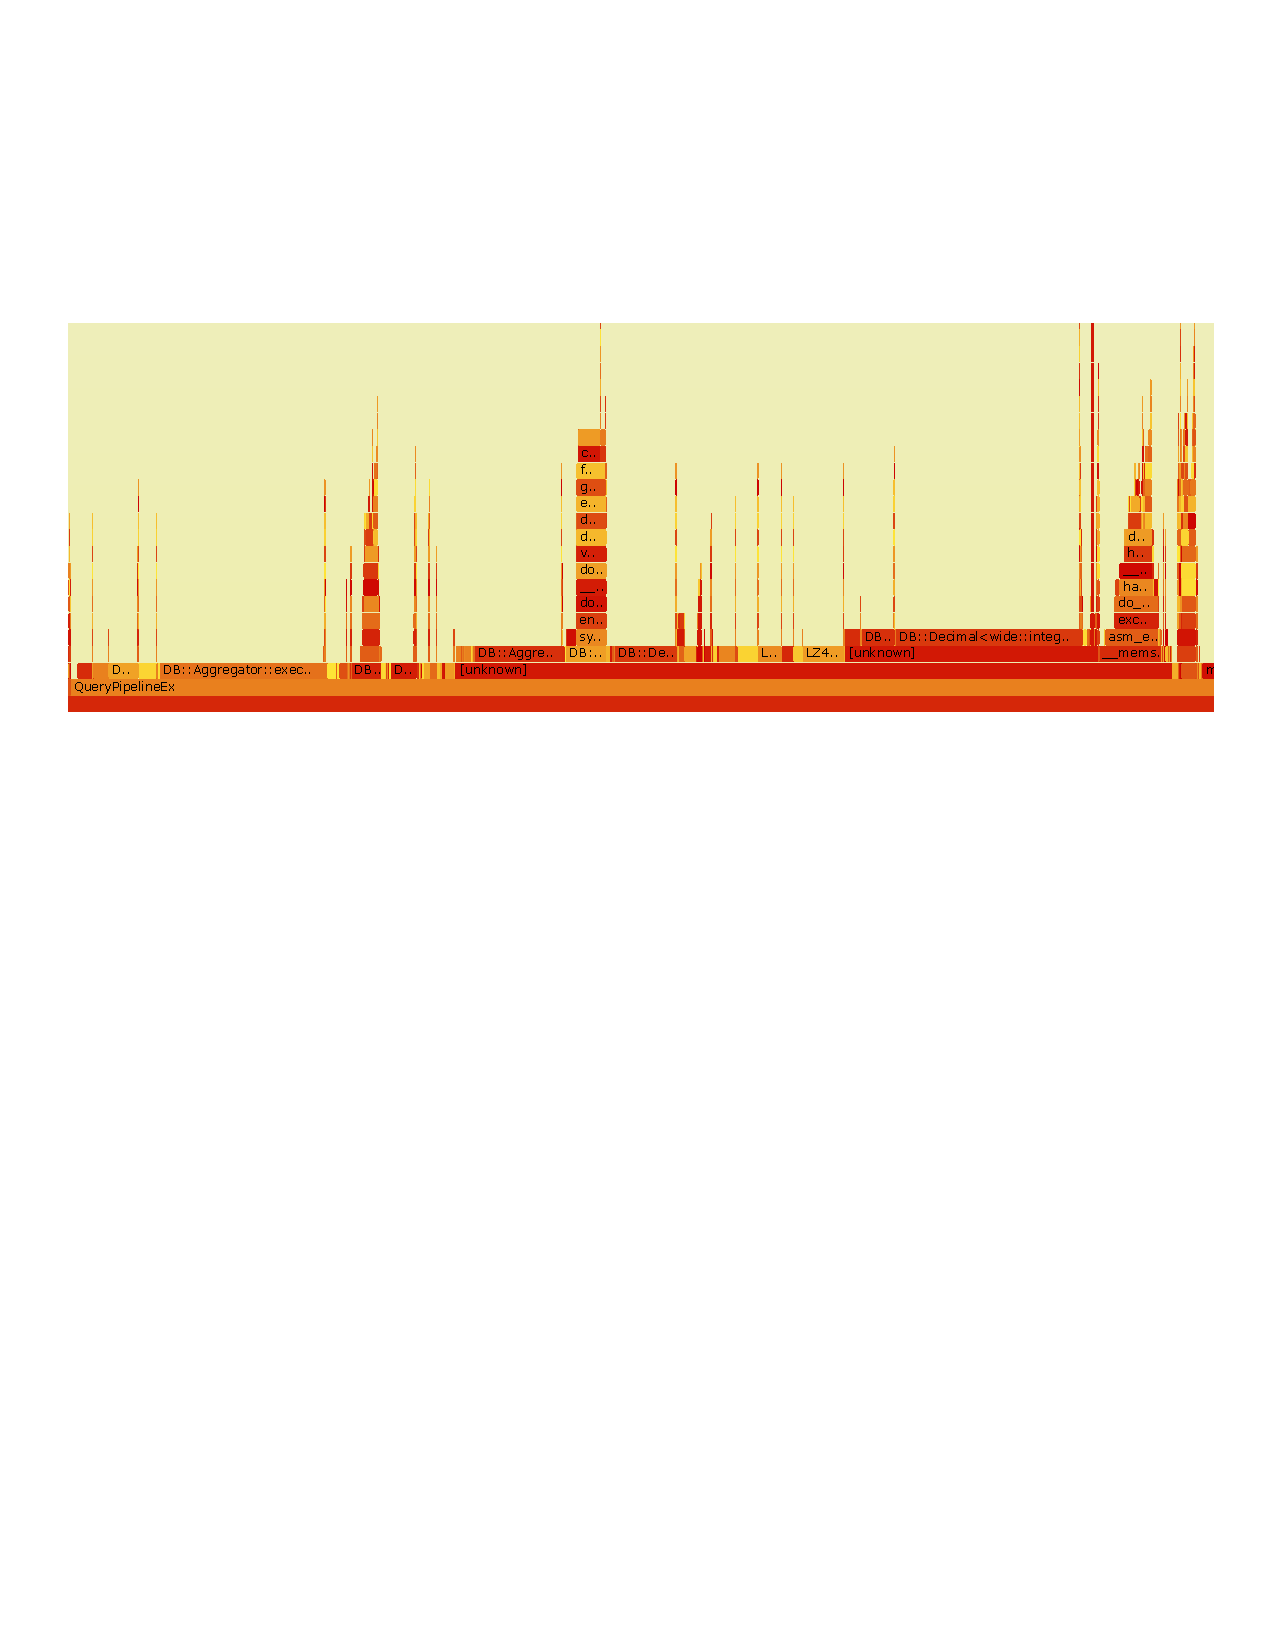
\includegraphics[width=\columnwidth]{img/flamegraph.pdf}
\caption{Flamegraph of ClickHouse Server showing syscall overhead}\label{fig:profiling}
\end{figure}

ClickHouse's \texttt{MergeTree} engine exemplifies this cross-domain problem, as shown in the profiling data in Figure~\ref{fig:profiling}. A typical OLAP query in ClickHouse follows this path: client query → column-file reads (\texttt{pread()}) → distribution to remote shards (\texttt{send()}) → network stack → remote node's \texttt{recv()} → disk lookup → response aggregation. Its columnar storage engine issues large numbers of small, random \texttt{read()} calls against compressed column files and mark-file offsets, with each compressed-block fetch and metadata lookup translating into a user-kernel transition. In distributed setups, remote-shard requests add further \texttt{send()} and \texttt{recv()} calls for data fetches and Raft heartbeats. Our profiling shows that the blocking \texttt{read()} syscall alone consumes ~25\% of query time, while small network receives (heartbeats, shard updates) account for another ~2\%. The cumulative cost of these syscalls—exacerbated by Spectre/Meltdown mitigations—introduces tens of microseconds of overhead per transition, multiplying into hundreds of milliseconds on fan-out queries. When a query spans dozens of remote partitions, each extra transition adds up quickly, creating a critical bottleneck for interactive dashboards and real-time analytics that cannot be solved by optimizing either storage or networking in isolation.

We introduce \sys, a unified syscall-chaining framework that bridges both domains. Our solution dynamically rewrites POSIX I/O calls into batched submissions, unifies memory management across domains through shared regions, coordinates cross-domain operations while preserving correctness, and adaptively optimizes for tail latency. \sys requires no application modifications, achieving significant performance gains by eliminating redundant context switches and memory copies.

\section{\sys Design}\label{sec:design}

We introduce \sys (Figure~\ref{fig:bur}) to address these challenges by seamlessly unifying both domains. Our architecture creates an end-to-end bypass path that transparently intercepts, batches, and chains disk and network operations without application modifications. Through a combination of dynamic binary rewriting and in-kernel eBPF programs, we eliminate redundant context switches while maintaining POSIX semantics. The system consists of three tightly-integrated components that work together to optimize cross-domain I/O flows for modern analytical workloads.

\begin{figure}[h]
\centering
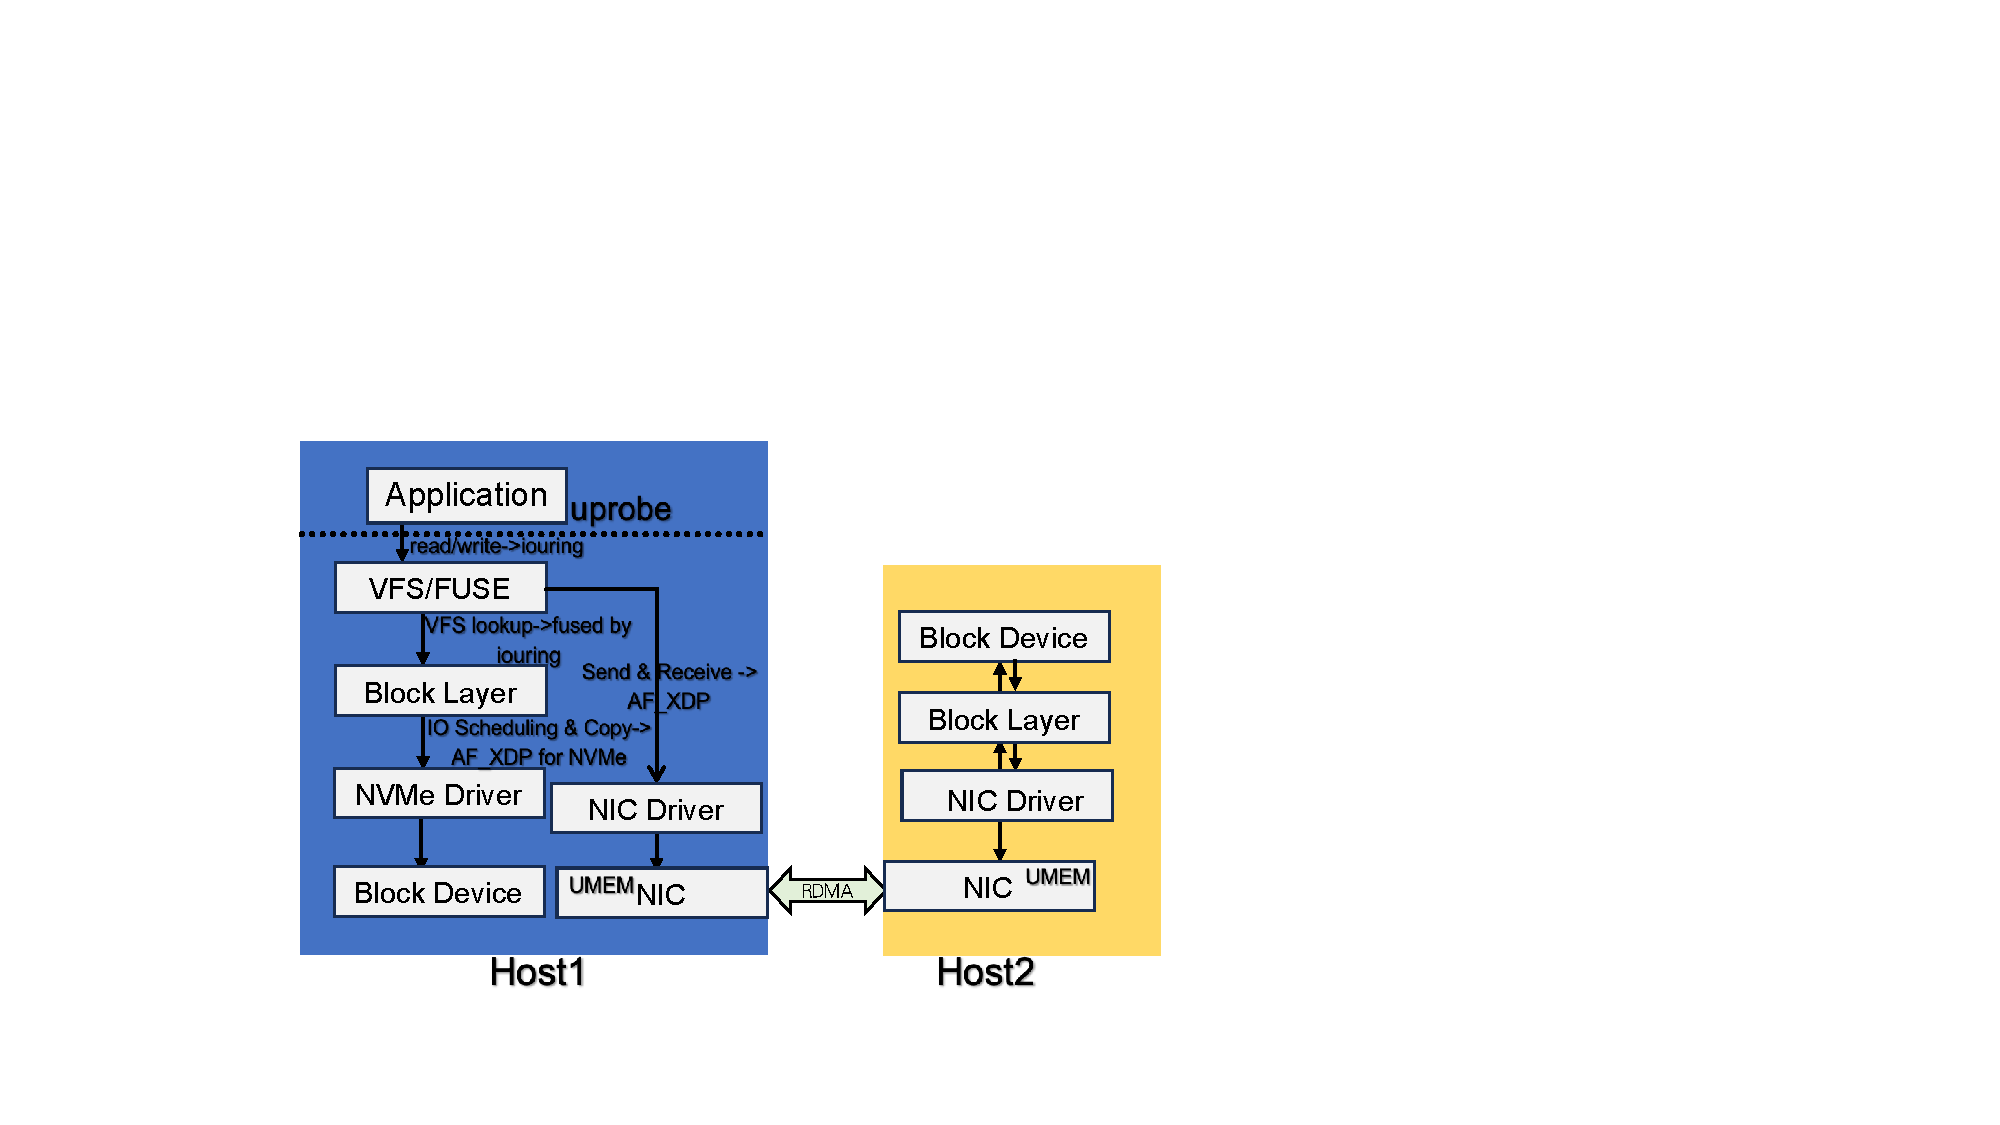
\includegraphics[width=\columnwidth]{img/bur.pdf}
\caption{\sys Architecture for ClickHouse}\label{fig:bur}
\end{figure}

\textbf{Syscall-Chaining Engine.} We dynamically intercept POSIX I/O calls and redirect them into unified rings using binary rewriting and eBPF. The engine automatically rewrites ClickHouse's invocations of \texttt{read()}, \texttt{send()}, and \texttt{recv()} into batched \texttt{io\_uring} submissions using bpftime-like uprobes, eliminating redundant transitions. By placing probes at key ClickHouse functions (e.g., \texttt{MergeTree::readMark()}, \texttt{MergeTree::readData()}), we maintain semantic context across syscall boundaries, preserving correct ordering and dependencies. The eBPF verifier ensures no infinite loops or memory violations, with explicit rollback paths for upgrades or verification failures, guaranteeing system stability even during live patching operations.

\textbf{Cross-Domain Ring Bridge.} The heart of \sys is a novel ring design that unifies storage and network operations through shared memory. We use BPF maps to bridge user-space \texttt{io\_uring} rings and in-kernel XDP processing, allowing both to access a common zero-copy region without intermediate copies. This approach requires a unified descriptor format that encompasses both disk SQEs (\texttt{io\_uring} descriptors) and network SQEs (XDP frame metadata), enabling atomic operations across domains. Critically, our descriptor metadata includes cross-domain dependency information, enabling in-kernel coordination of chained operations without user intervention—for example, automatically triggering a network send once a disk read completes, all without returning to user space.

\textbf{Tail-Latency Optimizations.} To ensure consistent performance even under load, we implement several techniques specifically targeting tail latency in analytical workloads. Our user-space coordinator monitors operation latency and adjusts batch sizes dynamically, flushing smaller batches under high load. For example, during high query concurrency, we dynamically reduce batch sizes for critical path operations to bound 99th-percentile latency by 150us. We also implement priority-aware scheduling that detects latency-sensitive operations (e.g., metadata lookups vs. large column scans) and prioritizes their execution, with NURaft heartbeat traffic receiving highest priority to maintain replication stability. For urgent requests, a lightweight BPF program can preempt in-progress operations and expedite high-priority traffic, improving worst-case tail latency by up to 45\% compared to default first-come-first-served processing.

\section{Implementation}\label{sec:implementation}

We implemented \sys in ~2000 lines of C/C++ and eBPF code, focusing on the ClickHouse use case while maintaining compatibility with unmodified binaries.

\paragraph{UMEM Management}
We allocate a contiguous user-space memory region (UMEM) and register it with both the kernel's \texttt{io\_uring} subsystem and the AF\_XDP driver. This shared region eliminates copies between disk and network paths. For \texttt{io\_uring}, these pages hold direct DMA buffers for NVMe reads and writes, significantly reducing data movement overhead. For AF\_XDP, the same pages serve as zero-copy packet buffers, enabling efficient network transmission without redundant copying. A custom slab allocator manages the complete buffer lifecycle across domains, ensuring proper resource utilization and preventing memory leaks as buffers transition between storage and network subsystems.

\paragraph{eBPF Program Coordination}
Three key eBPF programs coordinate the cross-domain operations. The syscall interceptor attaches to \texttt{sys\_read}, \texttt{sys\_send}, and related syscall entry points to redirect operations into our unified processing path. The XDP packet router steers select network traffic into the shared UMEM region, distinguishing between traffic that requires our optimized path and regular traffic that can follow the conventional network stack. The IO completion handler triggers dependent operations when prerequisites complete, maintaining the causal relationships between operations without requiring application intervention or additional context switches.

\paragraph{ClickHouse Integration}
For ClickHouse, we focus on optimizing the MergeTree storage engine and distributed query paths. Compressed column file reads in \texttt{MergeTree} are intercepted via USDT probes, allowing us to capture both data and metadata operations with minimal overhead. Distributed query traffic and Raft heartbeat messages are redirected through AF\_XDP, prioritizing low-latency communication for both data transfer and cluster consistency. Data compression and decompression operations remain untouched to maintain compatibility with existing codebases and storage formats, ensuring that our optimization layer integrates seamlessly with the existing ClickHouse ecosystem.

\section{Preliminary Evaluation}\label{sec:evaluation}

We evaluated \sys on ClickHouse (v21.8) running on CloudLab servers with Intel Xeon Silver 4314 CPUs, 128GB RAM, and dual-port 100Gb Mellanox ConnectX-6 NICs. Each server has a Samsung PM1725a NVMe SSD.

\paragraph{TPC-H Performance}. We measured performance using TPC-H at scale factor 20 on a single NVMe-SSD, comparing our SQPOLL + HugePage + Registered-File configuration against a Thread-poll + pread baseline. For I/O-bound queries such as Q6, average latency improves by up to 23\%, decreasing from 0.637s to 0.490s. When running a narrow column scan (SELECT SUM(LENGTH(l\_comment))), latency improves by 27.3\%, dropping from 0.616s to 0.447s. Row throughput increases by up to 39\% for I/O-dominated workloads, directly reflecting the elimination of syscall and context switch overhead. Most critically, 99th-percentile latency for short-running metadata queries improves by 3.2×, from 25.4ms to 7.9ms, directly addressing the high-percentile latency outliers that impact interactive analytics and dashboard responsiveness.

\paragraph{Resource Utilization}. Profiling shows where \sys eliminates overhead throughout the I/O path. Context switch overhead is reduced by up to 85\%, reflecting our ability to batch and chain operations that would normally require separate system calls. Memory copy operations are reduced by up to 73\% through our zero-copy architecture and shared memory regions. CPU utilization is lowered by 30\% at equivalent throughput, freeing cores for additional application logic or increased query concurrency. Tail latency (p99) for distributed sharding operations drops by 68\%, enabling more predictable query response times even under varied workload conditions. For I/O-dominated workloads like SELECT SUM(LENGTH(l\_comment)), data throughput nearly doubles from 251.5MB/s to 475.5MB/s as zero-copy bypass and batching eliminate copy and syscall overhead. Under mixed scan-metadata workloads, our adaptive batching heuristic maintains 99th-percentile latency below 10ms, compared to 35ms with standalone \texttt{io\_uring} and 42ms with native syscalls.

\bibliographystyle{plain}
\bibliography{cite}

\end{document}